%-------------------------------------------------------------------------------
\chapter{Motivations}
\labelchapter{ch.problem}

\renewcommand{\labelitemi}{$-$}

%-------------------------------------------------------------------------------

%%%%%%%%%%%%%%%%%%%%%%%%%%%%%%%%%%%%%%%%%%%%%%%%%%%%%%%%%%%%%%%%%%%%%%%%%%%%%%%%
%%%%%%%%%%%%%%%%%%%%%%%%%%%%%%%%%%%%%%%%%%%%%%%%%%%%%%%%%%%%%%%%%%%%%%%%%%%%%%%%

\lettrine[lines=2]{T}{his} chapter introduces the problematic of this thesis, as well as the issues and challenges at stake in this work.
Important considerations are discussed to highlight some interrogations that will be answered throughout this manuscript.

To begin with, we introduce the notion of hardware acceleration, with a particular focus on how \myLongAcs{FPGA}{Field-Programmable Gate Array} can be used to build hardware accelerators.
We then expose the standard design methodologies to discuss their limitations, and introduce the \myLongAc{DSE}{Design Space Exploration} processes as a way to increase the productivity of hardware developers.
Finally, we discuss the usage of a new development paradigm --- known as \myLongAc{HCL}{Hardware Construction Languages} --- to cope with the limitations of the standard design methodologies, and how it can be used for efficient \myAc{DSE} implementations.

\vspace*{\fill}
\minitoc 
\mtcskip 

\newpage
%%%%%%%%%%%%%%%%%%%%%%%%%%%%%%%%%%%%%%%%%%%%%%%%%%%%%%%%%%%%%%%%%%%%%%%%%%%%%%%%

\section{Hardware Design}
\label{ch.problem:sec.hardware}

    \subsection{Hardware Acceleration}
    \label{ch.problem:sec.hardware:ssec.acceleration}
        While people are growing familiar with the concept of generic purpose \myLongAcs{CPU}{Central Processing Unit} integrated in their embedded devices and computers, they might not be familiar with the notion of hardware acceleration.
        Hardware accelerators are digital circuits built to cope with the limitations of \myAcs{CPU}, \ie insufficient energy efficiency or performance, and can be found in many application domains ranging from image processing to network filtering.
        They relies on a particular trade-off between a circuit efficiency and its programmability: \myAcs{CPU} can be programmed for every possible usage manipulating digital data, but an \myLongAc{ASIC}{Application-Specific Integrated Circuit} implementing a given algorithm will perform way faster than a \myAc{CPU} providing the same functionality, and consume way less energy --- however the \myAc{ASIC} function is fixed.

        Other accelerators do exist on this programmability {\tn vs} performance range, varying from domain specific processors such as \myLongAcs{GPU}{Graphical Processing Unit} or \myLongAcs{DSP}{Digital Signal Processor} to (re)configurable circuits, based on fabrics of basic operators that can be (re)programmed to perform any operation, providing an interesting trade-off between programmability and performance/energy efficiency.

        Domain specific processors are promising candidates for hardware acceleration, as programming processes are similar to software development.
        Usages are evolving to cope with hardware acceleration needs --- \eg \myAcs{GPU} are now used in many computation intensive algorithm acceleration beside graphical processing, using particular programming patterns (such as matrix operations) to take advantage of the inherent structure of the hardware.
        However, such development processes are limited to particular usages (either domain specific algorithm or particular patterns), and are thus not appropriate for every usages.

        On the other hand, digital circuits (such as \myAcs{ASIC} or configurable circuits), require specific development processes, known as {\bf hardware development processes}.
        In this context, configurable circuits are also to be considered when building hardware accelerators, as their programmability allows evolution abilities while offering performances and energy efficiency orders of magnitude better than \myAc{CPU} implementations.
        Among them, \myLongAcs{FPGA}{Field-Programmable Gate Array} --- digital chips built as arrays of reconfigurable basic blocs --- are commonly used for hardware acceleration.
        However, developing a hardware accelerator for a given algorithm requires expertise about the target, as an \myAc{ASIC} implementation is way different from a \myAc{FPGA} one, and specific knowledge is to be brought by the developer in order to develop efficient circuits.
        Hardware design is thus a time consuming task which requires a lot of effort and expertise, and initiatives are taken to ease and accelerate the work of hardware developers.
    \subsection[FPGAs as Hardware Accelerators]{{\it Field-Programmable Gate Arrays} as Hardware\\Accelerators}
        \label{ch.problem:sec.hardware:ssec.fpga}

            As \myAcs{FPGA} offer interesting performances for hardware implementation while remaining more programmable than \myAcs{ASIC}, they have been used as hardware accelerators for a long time, and keep providing promising circuits in various domains, such as network filtering \cite{bruant_towards_2021},  neural network implementations \cite{nurvitadhi_can_2017} or DNA sequencing \cite{di_tucci_architectural_2017}.

            \begin{figure}[h!]
                \centering
                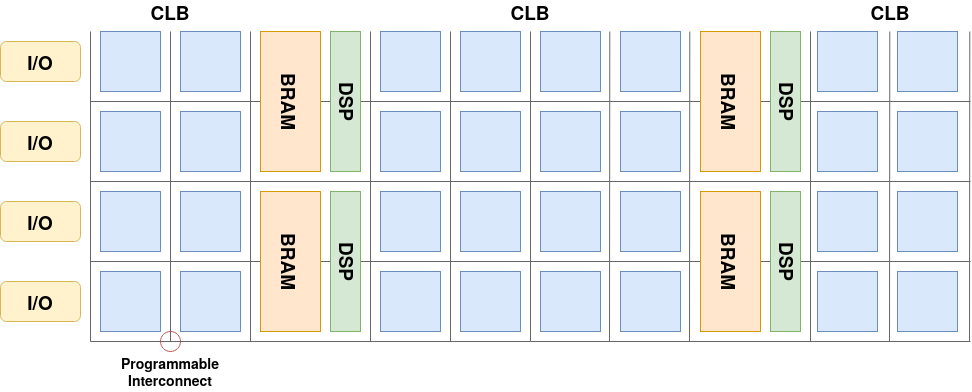
\includegraphics[width=1.0\textwidth]{Figures/FPGA-Structure.png}
                \caption[Xilinx Virtex 7 FPGAs structure]{Simplified schematic of Xilinx Virtex 7 FPGAs structure}
                \label{ch.problem:sec.hardware:ssec.fpga:sssec.fpga:fig.structure}
            \end{figure}
            \begin{figure}[h!]
                \centering
                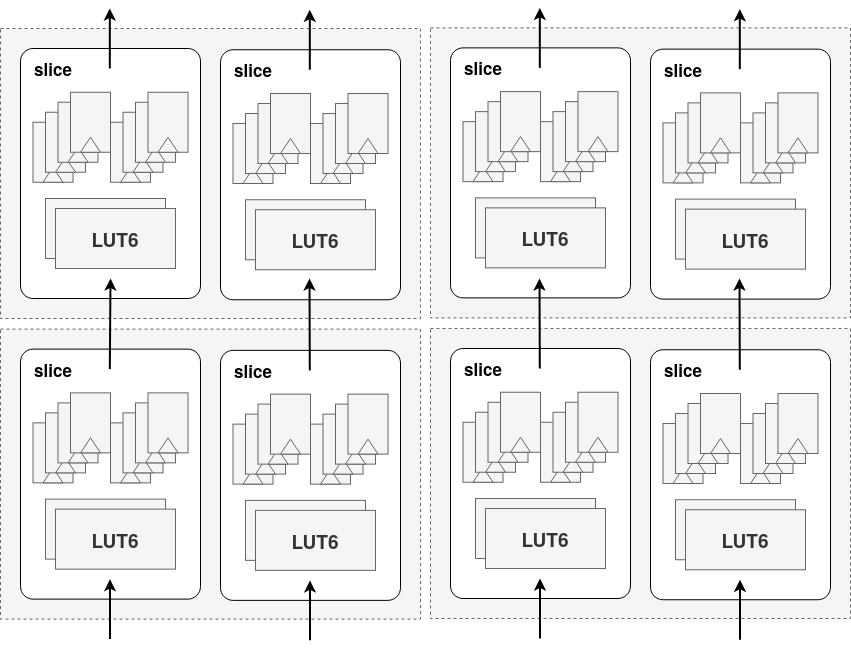
\includegraphics[width=0.8\textwidth]{Figures/FPGA-CLB.png}
                \caption[Xilinx Configurable Logic Blocks]{\myLongAcs{CLB}{Configurable Logic Block}: Xilinx FPGAs basic blocks}
                \label{ch.problem:sec.hardware:ssec.fpga:sssec.fpga:fig.clb}
            \end{figure}

            In order to build efficient design methodologies for \myAc{FPGA} based accelerators, one must understand board structures to comprehend technological specificities.
            Figure \ref{ch.problem:sec.hardware:ssec.fpga:sssec.fpga:fig.structure} introduce a simplified structure of a Xilinx \myAc{FPGA} as an example.
            As can be remarked, the structure is inherently heterogeneous, area being distributed between \myLongAcs{IO}{Input/Output block}, \myLongAcs{CLB}{Configurable Logic Block}, \myLongAcs{DSP}{Digital Signal Processor} and \myLongAcs{BRAM}{Block RAM}.
            Digital functions are based on \myAcs{CLB} (Fig. \ref{ch.problem:sec.hardware:ssec.fpga:sssec.fpga:fig.clb}, as defined in \cite{xilinx_clb_2016}) that include both computation resources with \myLongAcs{LUT}{Look-Up Table} and memory resources with \myLongAcs{FF}{Flip Flop}, but \myAc{DSP} blocks can be used to perform specific computations like multiplications, and \myAc{BRAM} can be used as embedded memory to offer large memories with low access latency.
            At least four different resources are thus to be considered when developing a hardware accelerator for such target --- \myAc{LUT}, \myAc{FF}, \myAc{DSP} and \myAc{BRAM} --- depending on both objectives and constraints of the problem.

            Nowadays, most of \myAcs{FPGA} are integrated in various \myLongAcs{SoC}{Systems on Chip}, tightly coupled with \myAcs{CPU} and other peripherals.
            However, in the context of this work, we will only consider \myAc{FPGA} implementation of different algorithms, and try to ease the life of \myAc{FPGA} developers, with no further focus on the integration of the accelerators.

            Such considerations raise the first interrogations of this manuscript: 
            \mdr{
                \begin{itemize}
                    \item How can we ease hardware development ?
                    \item How can we integrate \myAcs{FPGA} specific constraints in hardware\\design methodologies ?
                \end{itemize}
            }

    \subsection{Standard Paradigms}
    \label{ch.problem:sec.hardware:ssec.paradigms}
        As circuit complexity (\ie number of transistors used in a chip) is growing exponentially, as stated by {\bf Gordon Moore's law} in 1965 \cite{moore_cramming_1965}, hardware designs methodology are bound to evolve and exhibit high level abstraction to developers to cope with the scaling of \myLongAc{VLSI}{Very Large Scale Integration}. 

        First languages developed to describe hardware circuits by abstracting low level considerations were \myLongAcs{HDL}{Hardware Description Language} such as VHDL and Verilog.
        Originally developed for hardware simulation, working at \myLongAc{RTL}{Register-Transfer Level} --- \ie considering data signal as entity instead of considering physical implementation details such as transistor layout and power supply --- their aim was to raise the abstraction level and allow design of large scale circuits.
        To do so, they allow to describe complex circuits by combining behavioural descriptions (how digital signals are behaving in the circuit, often used to describe basic modules with simple functionalities), and structural descriptions (how are basic blocks interacting).
        \myAc{HDL} classic development processes are quite straightforward, as can be seen in Figure \ref{ch.problem:sec.hardware:ssec.paradigms:fig.rtl} (as translated from Prost-Boucle's thesis \cite{prost-boucle_generation_2014}), consisting in manual translations of sequential algorithm to hardware description of the functionality.
        Circuit descriptions are then fed to a set of time consuming software --- including {\bf synthesis} and {\bf place and route} steps --- in order to translate such high level descriptions to physical representations that can be used to program \myAcs{FPGA}.
        Moreover, in order to comply with design constraints and objectives, such process requires manual iterations to find an acceptable fit, and each iteration can be expensive due to the complexity of both synthesis and place and route processes, and may require manual modifications of the original design, which can be both time consuming and error prone tasks.
        
        \begin{figure}[h!]
            \centering
            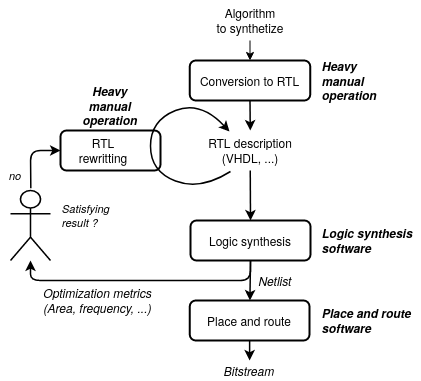
\includegraphics[width=0.8\textwidth]{Figures/HDL-flow.png}
            \caption{Example of RTL design flow}
            \label{ch.problem:sec.hardware:ssec.paradigms:fig.rtl}
        \end{figure}

        \newpage
        Another approach for easing hardware development is based on \myLongAcs{DSL}{Domain Specific Language}.
        \myAcs{DSL} are languages leveraging prior knowledge about the application domains (what are the important operations to perform, what data patterns are frequently used, ... \ie what domain specific optimizations can be performed) to build efficient mapping for acceleration.
        In this way, this approach differs from \myAc{DSP} usage, as the goal is not to program specific processors but rather build generic circuits --- \eg on \myAc{ASIC} or \myAc{FPGA} --- using specificity of a particular domain.
        A typical \myAc{DSL} development flow (quite similar to \myAc{HDL} ones) is presented in Figure \ref{ch.problem:sec.hardware:ssec.paradigms:fig.dsl}. 
        Using domain specific knowledge allow easier writing and refinement of the \myAc{DSL} code base, compared to \myAc{HDL} programming, resulting in faster iteration steps, and feedback generations can also be enhanced by using pre-synthesis estimations based on \myAc{DSL} operations, producing faster development methodologies.
        In fact, providing early estimations of iteration metrics --- \eg area and frequency --- is a common technique to accelerate development flows by reducing the time dedicated to synthesis and place and route steps, and it was used as used as a basis of one of the main initiatives for easier development: \myLongAc{HLS}{High Level Synthesis}.
        \begin{figure}[h!]
            \centering
            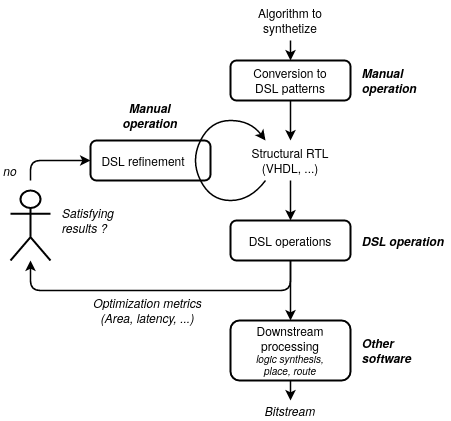
\includegraphics[width=0.8\textwidth]{Figures/DSL-flow.png}
            \caption{Example of DSL design flow}
            \label{ch.problem:sec.hardware:ssec.paradigms:fig.dsl}
        \end{figure}

        \myAc{HLS} methodologies have been developed to close the gap between software developers and hardware designers.
        It is based on a modification of the entry point of the whole process, as it does no longer require to use hardware specific languages such as \myAcs{HDL} or \myAcs{DSL}, but rather uses standard software languages such as {\bf C language} to describe the target algorithm, and then relies on a translation tool that compiles this algorithmic approach to a hardware description at \myAc{RTL} level.
        Figure \ref{ch.problem:sec.hardware:ssec.paradigms:fig.hls} (also translated from Prost-Boucle's thesis \cite{prost-boucle_generation_2014}) introduces a classical \myAc{HLS} based design flow, operating on an intermediate representation issued from the compilation of the input algorithm to perform optimization-estimation steps until given constraints and objectives are respected.
        Manual interventions of the developer are reduced as the software is able to modify the generated circuits in order to optimize the design, but can be needed in order to guide the tool by adding specific knowledge --- using optimization directives (such as {\bf C pragmas}) directly in the algorithm description to define memory patterns or exhibit parallelism for example.
        This feature allows to close the performance gap with \myAc{HDL} design flows, but as it requires specific hardware knowledge, it can no longer directly be used by software neophytes and require prior skill improvement.
        
        \begin{figure}[h!]
            \centering
            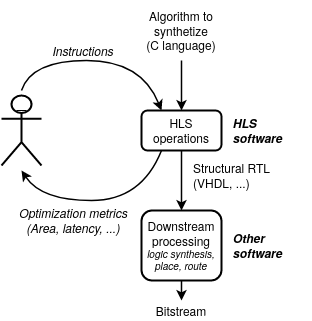
\includegraphics[width=0.68\textwidth]{Figures/HLS-flow.png}
            \caption{Example of HLS design flow}
            \label{ch.problem:sec.hardware:ssec.paradigms:fig.hls}
        \end{figure}

        A quick review of standard paradigms for hardware development hence exhibits some interrogations about classical design methodologies:
        \mdr{
            \begin{itemize}
                \item What are the strength of standard paradigms for hardware\\development ?
                \item What are their limitations ?
                \item How can we ease hardware development processes ?
            \end{itemize}
        }

    \subsection[Hardware Construction Languages]{Addressing Standard Paradigms Limitations through {\it Hardware Construction Languages}}
    \label{ch.problem:sec.hardware:ssec.hcl}
        Standard paradigms for hardware development have evolved the last decade in order to cope with the needs of faster development methodologies and close the gap with software processes.
        However, such methodologies present limitations that one should try to overcome in order to ease the life of hardware developers.
        \myAc{HDL} development requires time consuming and error prone processes, and does not allow easy component re utilization, as evolving a design for a new use case require heavy manual modification of the base code. 
        On the other hand, \myAc{HLS} methodologies can accelerate development processes, and code re utilization is easier as the base code is lighter than with \myAcs{HDL} --- nonetheless, modifying an existing accelerator requires an advanced knowledge of inserted directives which may not be intuitive, and the whole process relies on automatic tool inferences.
        Algorithmic compilation toward hardware description is a difficult problem, as it implies a change of paradigm, from a sequential representation of the algorithm toward a behavioural definition of a circuit. 
        In order to do so, the tool is taking decision that are usually taken by expert developers in standard \myAc{HDL} methodologies that may generate non optimal designs, and wrong directive usage may accentuate this flaw.
        Moreover, with the growing need of performance and efficiency, some of those decisions may be very specific to produce optimal utilization of available resources, and programming languages should allow developers to have full control over generated hardware --- and it cannot be done if automatic decisions are taken without the user knowing it.
        In fact, \myAc{HLS} enables higher abstraction of circuits for design processes, but results in a lack of control over how those circuits are generated.
        As for \myAcs{DSL}, their usage is by-design limited to specific domains, and thus cannot be generalized as hardware development methodologies.

        To cope with those problems and improve the expressivity of developers while maintaining control over generated hardware, new paradigms are emerging, with \myLongAcs{HCL}{Hardware Construction Language} among them.

        \myAcs{HCL} are based on high level languages, allowing to build hardware generators instead of hardware circuits: instead of building a specific accelerators for a given task, such as a digital \myLongAc{FIR Filter}{Finite Impulse Response Filter} with 128 taps operating with 32 bits fixed point numbers, it can be used to build a parametrized \myAc{FIR Filter} generator that can be used to build various circuits, varying on the number of taps or the data type used for example. 
        To do so, they leverage high level features such as \myLongAc{OOP}{Object-Oriented Programming}, functional programming or reflexivity in order to provide more generic and reusable representations for hardware circuits.
        Moreover, as \myAcs{HCL} are working at \myAc{RTL} like standard \myAcs{HDL}, no performance/area overhead is introduced from using \myAc{HCL} over any other \myAc{HDL} \cite{izraelevitz_2017_reusability}, resulting in controllable generation of hardware implementations.
        Figure \ref{ch.problem:sec.hardware:ssec.paradigms:fig.hcl} represents a typical \myAc{HCL} development flow, where the main difference with respect to standard paradigms is that both generator description and parameters definition are exposed by users, allowing to manage generated circuits while easing reuse and iteration over generated designs through exposed programming features.

        \myAcs{HCL} relies on \myLongAcs{HCF}{Hardware Construction Framework} to translate target-independent \myAc{RTL} code to technology dependent \myAc{RTL}, leveraging a compiler-like separation of concerns: using an \myLongAc{IR}{Intermediate Representation} of circuits to perform optimization and code generation, target specific concerns are decorrelated from \myAc{HCL} description as they can be managed directly by operating on the \myAc{IR}.
        Common \myAcs{HCL} use high level languages such as \scala{} for \myLongAc{Chisel}{Constructing Hardware in a Scala Embedded Language} \cite{bachrach_chisel_2012}, {\bf python} for PyMTL \cite{lockhart_pymtl_2014} or {\bf Haskell} for C$\lambda$ash \cite{baaij_clash_2010}.

        As \chisel{} is a promising \myAc{HCL}, with state of the art implementations from both academic and industrial worlds, such as in-order and out-of-order RISC-V implementations \cite{celio_berkeley_2015} \cite{asanovic_rocket_2016} or Google latest \myLongAc{TPU}{Tensor Processing Unit} \cite{google_tpu_2018}, it will be used as an example of \myAc{HCL} in this work.
        \chisel{} development flow is quite similar to standard \myAc{HDL} flows as it relies on the same tool set to generate both constraint and objective metrics and resulting bitstream --- in fact \chisel{} is integrated in standard \myAc{HDL} flows by generating structural \myAc{RTL} (\tn{Verilog}) code after what is called the emission phase (\ie building a non parametrized hardware circuit from the corresponding hardware generator).
        However, as both hardware generator notion and high level programming features for hardware development are recent progresses, improvements of \myAc{HCL} based methodologies are still to be proposed.

\clearpage
        \begin{figure}[h!]
            \centering
            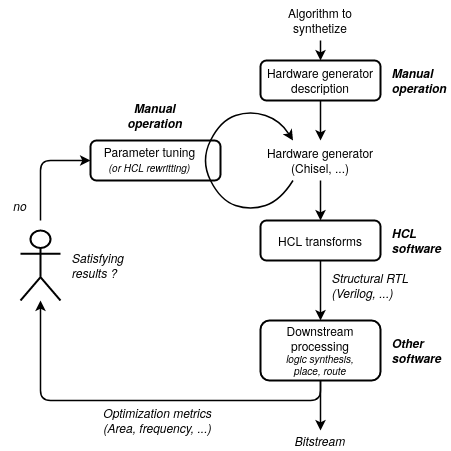
\includegraphics[width=0.83\textwidth]{Figures/HCL-flow.png}
            \caption{Example of HCL design flow}
            \label{ch.problem:sec.hardware:ssec.paradigms:fig.hcl}
        \end{figure}

        Emergence of \myAc{HCL} paradigm hence raises few interrogations on the improvement that new technologies and methodologies can bring to the industry of semi-conductor:
        \mdr{
            \begin{itemize}
                \item How can \myAcs{HCL} cope with standard paradigms limitations ?
                \item How can high level programming features be used in hardware\\development ?
                \item What can \myAcs{HCL} bring to hardware developers ?
                \item How can \myAcs{HCL} flow be improved for easier iterations over generated designs ?
            \end{itemize}
        }

        Moreover, as \chisel{} will be used as a basis for this work, an analysis of its interesting features is provided in Appendix \ref{app.chisel}. It should help readers to understand the opportunities brought by the \myAc{HCL} paradigm, using simple examples of \chisel{} usage to expose differences from standard \myAcs{HDL}.


%%%%%%%%%%%%%%%%%%%%%%%%%%%%%%%%%%%%%%%%%%%%%%%%%%%%%%%%%%%%%%%%%%%%%%%%%%%%%%%%

\clearpage
\section{Design Space Exploration}
\label{ch.problem:sec.dse}

    \subsection{Definitions and Interests}
    \label{ch.problem:sec.dse:ssec.definitions}

    It may seem counter intuitive, but hardware designers expertise is more about decision making than describing circuits.
    As a matter of fact, implementing a particular algorithm for a given target can be done in a lot of different ways, and it is up to the developer to choose among different implementation options to build optimal circuits with respect to its use case.
    However, even with senior expertise, optimal solutions may not be trivial, and developer may not even consider them in the process, resulting in suboptimal designs.
    
    To cope with this problem, \myLongAc{DSE}{Design Space Exploration} methodologies have emerged, allowing exploration and comparison of implementation options at different granularity levels --- options can vary from basic operation implementations such as multiplication algorithm, to global parameters, such as parallelism level of the design.
    A design space is defined as the set of every possible implementation candidate for a given algorithm, and as implementation options may grow exponentially with circuit complexities, exhaustive exploration processes may be unfeasible in an acceptable amount of time.
    Due to that, more complex exploration strategies were built to reduce space traversal, thus reducing exploration time while maintaining satisfying \myLongAc{QoR}{Quality of Results}, \ie finding implementations with performances comparable to a global optimal implementation as could be found from exhaustive space traversal. 

    However, one cannot define a generic, optimal solution for exploration, as a lot of parameters are both target and algorithm specific \cite{schafer_high-level_2020}.
    Moreover, design space definition is not trivial either, as defining the implementation options require either automatic tool inferences, or programming expressivity for developers to bring their expertise in the process.
    Ergo, \myAc{DSE} methodologies remain a prolific search domain, and standard approaches are continuously being improved --- raising even more interrogations:

    \mdr{
        \begin{itemize}
            \item What does \myAc{DSE} bring to hardware developers ?
            \item Which features are necessary for efficient \myAc{DSE} ? 
            \item Which features could be useful ?
        \end{itemize}
    }

\clearpage
    \subsection{Standard Approaches}
    \label{ch.problem:sec.dse:ssec.approaches}

    As exhaustive exploration remains impracticable for complex circuits, more clever exploration strategies were developed to fasten exploration processes. 
    In order to do so, one of the main approach is based on {\bf Pareto optimal solutions} \cite{schafer_high-level_2020}: considering both a performance and a cost metric, Pareto optimal solutions are implementations that are optimal in their neighbourhood, meaning that modifying a parameter will result in either a more costly or a less performant solution.
    The goal is thus to build algorithm to approximate the Pareto frontier without exhaustive traversal of the design space, resulting in optimal design finding in a heavily reduced amount of time.
    Figure \ref{ch.problem:sec.dse:ssec.definitions:fig.pareto} introduce a classical, Pareto based \myAc{DSE} methodology, using resource usage (which can be amount of transistor, of \myAc{LUT}, of \myAc{DSP}, ...) as a cost metric, in order to find best implementations under both resource and performance constraints. 
    It enables design space partitioning to exhibit a reduced number of implementations to developers, helping them in the design process, as they can now choose among a set of implementations with a warranty that they did not miss potentially optimal solutions.

    \begin{figure}[h!]
        \centering
        % includes here
\usetikzlibrary{patterns}

% style here

% figure here
\scalebox{1.25}{
\begin{tikzpicture}
\begin{axis}[
    xlabel={Resources},
    ylabel={Performance},
    axis lines = middle,
    x label style={at={(axis description cs:0.5,-0.01)},anchor=north},
    y label style={at={(axis description cs:-0.01,0.5)},rotate=90,anchor=south},
    xtick distance=1,
    ytick distance=1,
    yticklabels={,,},
    xticklabels={,,},
    xmin=0,xmax=5,
    ymin=0,ymax=5
]

\addplot [name path=curve,mark=none,smooth] coordinates{(1, 5) (1.01, 4.9) (1.1, 4) (1.25,3.2) (1.5,2.5) (2, 1.8) (2.5,1.45) (3, 1.25) (4, 1.07) (4.9, 1.01) (5, 1)};
\draw [name path=resource,red] (4, 0) -- (4, 5*\pgfkeysvalueof{/pgfplots/ymax}/6+0.05) node[right=0.2,rotate=-90] (resnode) {Resource constraint} -- (4, \pgfkeysvalueof{/pgfplots/ymax});
\draw [name path=performance,blue] (0, 3) -- (8*\pgfkeysvalueof{/pgfplots/xmax}/15, 3) node[above=0.1] (perfnode) {Performance constraints} -- (\pgfkeysvalueof{/pgfplots/xmax}, 3);
\addplot[fill=gray]fill between[of=curve and performance,soft clip={domain=1.3:4}];
\node (solution) at (2.85,2.32) {Suitable solutions};
\end{axis}
\end{tikzpicture}
}

        \caption[Pareto frontier representation]{Example of Pareto optimal solutions finding under resource and\\performance constraints}
        \label{ch.problem:sec.dse:ssec.definitions:fig.pareto}
    \end{figure}

    As shown in Figure \ref{ch.problem:sec.hardware:ssec.paradigms:fig.hls}, standard \myAc{HLS} development flows rely on \myAc{HLS} operations over generated circuit in order to generate acceptable solutions with respect to objective and constraints.
    To do so, \myAc{DSE} is used in most \myAc{HLS} tool as a medium to find acceptable solutions, varying implementation parameters from the original algorithm, such as loop unrolling, operation pipelining of memory partitioning: by giving freedom to the tool to make its own decision, a heavy design space is generated to compare a lot of different implementations.
    In order to reduce design space width, most flows thus use algorithms to approximate the Pareto frontier, using specific heuristics such as machine learning \cite{nardi_practical_2019} \cite{ferretti_leveraging_2020} or genetic algorithms \cite{manuel_model-based_2020}, and building efficient exploration strategies remains a trending search topic.
    Moreover, optimization directives can also be given to guide the exploration of the generated design space, resulting in efficient \myAc{DSE} processes.

    However, defining optimization directives requires user expertise, and automatic inferences about the design space and how to explore it may result in a lack of control of generated accelerators, which may lead to the impossibility to find the best fit --- especially on specific targets such as \myAcs{FPGA} where resource heterogeneity requires experience to produce clever decisions.

   Such considerations about standard \myAc{DSE} approaches bring interrogations about such processes:

    \mdr{
        \begin{itemize}
            \item What are the limitations of standard \myAc{DSE} approaches ? 
            \item Can \myAcs{HCL} help addressing those limitations ?
        \end{itemize}
    }

    \subsection{Limitations}
    \label{ch.problem:sec.dse:ssec.limitations}
        While standard \myAc{DSE} approaches have grown mature the last two decades --- especially with the rise of \myAc{HLS} tools --- limitations are still to be addressed to provide generic methodologies appropriate for every possible use cases.

        We discussed the challenge of building an interesting design space to explore, as automatic inferences of the tools used to generate implementation options allow multiple variations to be explored, but might result in an uncontrollable design generation in the end.

        Moreover, doing so, the generated design spaces are composed in a vast majority of known sub optimal solutions, as no particular expertise is used at design space generation step.
        It results in heavy design spaces that cannot be explored exhaustively, with the emergence of exploration strategies such as Pareto approximations to cope with the large amount of possible implementations, even if a lot of those implementations are not sound and would never be considered by a hardware developer.

        Last but not least, most of \myAc{DSE} tools define their own strategies, as well as metrics to optimize in the process, resulting in methodologies that are hard to adapt and reuse to any new use case.
        In fact, some particular use cases require to define specific metrics to optimize and consider, as well as particular exploration strategies, and tools should allow developers to bring their expertise and knowledge to the exploration process definition.
        For example, specific domains such as \myLongAc{AxC}{Approximate Computing} requires to consider the \myLongAc{QoS}{Quality of Service} of circuits in order to provide guarantees about the functionality of a design.
        However, most \myAc{DSE} tools does not allow users to add such metric in the exploration process, resulting in the need to use different flows to consider multiple metrics.

        In this context, one may wonder what can \myAcs{HCL} bring to hardware developers, especially in the context of \myAc{DSE}:
        \mdr{
            \begin{itemize}
                \item What can flexibility and genericity bring to \myAc{DSE} ?
                \item How can users define use case specific metrics ?
                \item How can users build custom exploration strategies ?
                \item How can \myAcs{HCL} be used for efficient \myAc{DSE} ?
            \end{itemize}
        }

%%%%%%%%%%%%%%%%%%%%%%%%%%%%%%%%%%%%%%%%%%%%%%%%%%%%%%%%%%%%%%%%%%%%%%%%%%%%%%%%

\section{Motivations and Organization}
\label{ch.problem:sec.synthesis}

    \subsection{Problem Statement}
    \label{ch.problem:sec.synthesis:ssec.summary}

        This chapter introduces the motivations of the work presented in this thesis.
        We discuss the role of \myAcs{FPGA} in the context of hardware acceleration, and expose various methodologies used to develop hardware accelerators relying on \myAcs{FPGA} specificities.
        Among them, we introduce \myAcs{HCL} as an emerging programming paradigm, and consider their usage to cope with standard paradigm limitations.
        We put a particular focus on \myAc{DSE} processes as a way to increase hardware developer productivity, and discuss \myAcs{HCL} usage to improve those processes.

\clearpage
        With respect to those considerations, the goal of this thesis is hence to answer those questions:
        \lmdr{
            \begin{itemize}
                \item How can \myAc{FPGA} designers productivity be improved\\using \myAcs{HCL} ?
                \item Which limitations of standard paradigms for hardware\\development can be addressed using \myAcs{HCL} ?
                \item How can \myAcs{HCL} be used for efficient \myAc{DSE} on \myAcs{FPGA} ?
            \end{itemize}
        }

    \subsection{Thesis Organization}
    \label{ch.problem:sec.synthesis:ssec.organization}
        In order to provide an intelligible analysis of the usage of \myLongAcs{HCL}{Hardware Construction Language} to build a flexible \myLongAc{DSE}{Design Space Exploration} framework that target \myLongAcs{FPGA}{Field-Programmable Gate Array}, this thesis is organized as follows.

        Chapter \ref{ch.state} outlines the related works of the literature on efficient \myAc{DSE} for \myAcs{FPGA}, as well as their limitations.
        Chapter \ref{ch.estimators} discusses the need of qualitative estimators to increase the developers productivity, and proposes interesting metrics to be considered in design and exploration processes, as well as relevant estimation methodologies to be used.
        Chapter \ref{ch.dse} introduces the usage of \myAc{DSE} in an \myAc{HCL} context, before exhibiting two complementary methodologies to exploit this paradigm in user defined custom strategies.
        In particular, a novel formalism for \myAc{DSE} is introduced in order to exhibit how the functional programming paradigm can be used to build intelligible and concise exploration strategies.
        Chapter \ref{ch.expe} exposes the experimental setup, including a software demonstrator integrating the defined methodologies and a benchmark of representative applications, and presents the results of the experimentations that were led.
        Chapter \ref{ch.conclusion} concludes this manuscript, discussing both the proposed contributions and the perspectives of evolution.

        In addition to those chapters, four appendixes are to be found at the end of this manuscript.
        Among them, Appendix \ref{app.chisel} provides some insights about the usage of \chisel, the chosen \myAc{HCL} for this work, which will help the reader to have a better apprehension of the features that such language can bring to the world of hardware design.

%%%%%%%%%%%%%%%%%%%%%%%%%%%%%%%%%%%%%%%%%%%%%%%%%%%%%%%%%%%%%%%%%%%%%%%%%%%%%%%%
%%%%%%%%%%%%%%%%%%%%%%%%%%%%%%%%%%%%%%%%%%%%%%%%%%%%%%%%%%%%%%%%%%%%%%%%%%%%%%%%
